\documentclass[../TinyBot.tex]{subfiles}
\begin{document}
    
\section{Motor} \label{sec:motor}
% gearbox, motor

To follow this guide it is not necessary to have an understanding of how motors work, though it may be interesting for you to learn. \href{https://www.explainthatstuff.com/electricmotors.html}{This} link has a good indepth explanation. 

\bigskip

Motors turn in proportion to the amount of current put through them. More current means a faster motor. 

When a motor stalls, it stops rotating. This happens when there is more force acting on the motor shaft than the motor can overcome. The stall current of a motor is the maximum current drawn when a motor stalls, in other words, applying its maximum torque - known as stall torque. \\

Similarly, free current is the current drawn when the motor is rotating freely, under no load. 

\bigskip


Each motor has a certain amount of torque it can provide, this depends greatly on the size and current draw of the motor. The speed of a motor also depends on the current going through the motor. 
% Gearboxes can be attached to a motor to increase the amount of torque provided, and change the rotations per minute (RPM) of the motor. 

% $TODO - Someone who knows about gearboxes, please complete this section. 
% \subsection{Gear Boxes}

\begin{minipage}[t]{0.6\textwidth}\vspace{0pt}

    To control the motor speed and torque, without controlling the amount of current going through the motor, 

    A gear box is useful for controlling the speed and torque outputs for motors. A motor has a maximum torque it can operate at before it starts to fail, this is known as a stall torque. If you want to increase the stall torque, you will need to lower the output speed, which can be accomplished with a gear box. The important factors to consider are the number of teeth of the gears for the input and output gears. The torque and speed are inversely proportional. The value of these ratios compared can be calculated as follows.\\
    
\end{minipage}
\begin{minipage}[t]{0.4\textwidth}\vspace{0pt}
    \begin{center}
        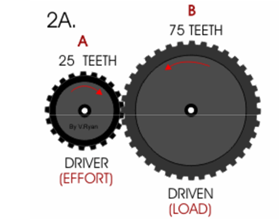
\includegraphics[width=\textwidth]{gear_labelled.png}
        \captionof{figure}{Driver and Driven Gear}
        \label{fig:gear-driver-driven}
    \end{center}
\end{minipage}


\[ R = \frac{N_1}{N_1} = \frac{D_1}{D_1} = \frac{\omega_2}{\omega_1} \]

Angular velocity = $\omega$, diameter of gear = D and number of teeth = N. Notice figure above, the more teeth an output gear has, the lower the angular velocity and larger the gear. It is worth noting that when there are only two gears, the output gear rotates in the opposite direction.


Now for calculating torque. \(T=F \times r\), where $F$ = force and $r$ = radius (usually we say $T = F*r*\sin(\theta)$, but since the gears are acting perpendicular to each other $\theta = 90^o$ i.e. $\sin{\theta} = 1$, therefore can be eliminated from the equation). This means the larger the output gear, the higher the torque. The torque of the input gear is supplied by a motor and the output torque is affected. \\

When connecting multiple gears, we call this a gear train. There are two types of gear trains, simple and complex. Simple gear trains are much like their name, simple. They connect next to each other and you only need to do the calculation for the first gear as an input gear and last gear as the output gear. These are useful for rapidly increasing torque or speed. Compound gear trains are slightly different and require a bit more thinking. A compound gear train means there can be multiple gears on the same shaft, meaning the gear ratio of the entire system will need to be calculated with each connecting gear and transfer the ratios through each individual shaft. You won’t have to deal with compound gear trains for this project, but feel free to investigate it more.
To summarise gears, the ratio of your input gear to output gear affects the characteristics of your output performance. If you want a higher torque use a larger output gear. If you want more speed, use a smaller output gear.

\begin{figure}[h]
    \centering
    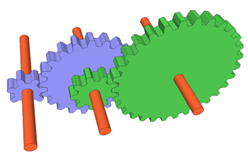
\includegraphics{compound_gears.png}
    \label{fig:gear-complex}
    \caption{Complex Gear Train}
\end{figure}


\end{document}